
%%%%%%%%%%%%%%%%%%%%%%%%%%%%%%%%%%%%%%%%%%%%%%%%%%%%%%%%%%%%%%%%%%%%%%%%%
                   % Capítulo 5: Manufactura e instrumentación          %
%%%%%%%%%%%%%%%%%%%%%%%%%%%%%%%%%%%%%%%%%%%%%%%%%%%%%%%%%%%%%%%%%%%%%%%%%


\chapter{\textcolor{Azul}{Manufactura e instrumentación}}

La figura (\ref{gripper01})                     %hace referencia a la imagen "planta" el número se inserta automáticamente
ilustra la geometría del efector final

\begin{figure}
	\centering
	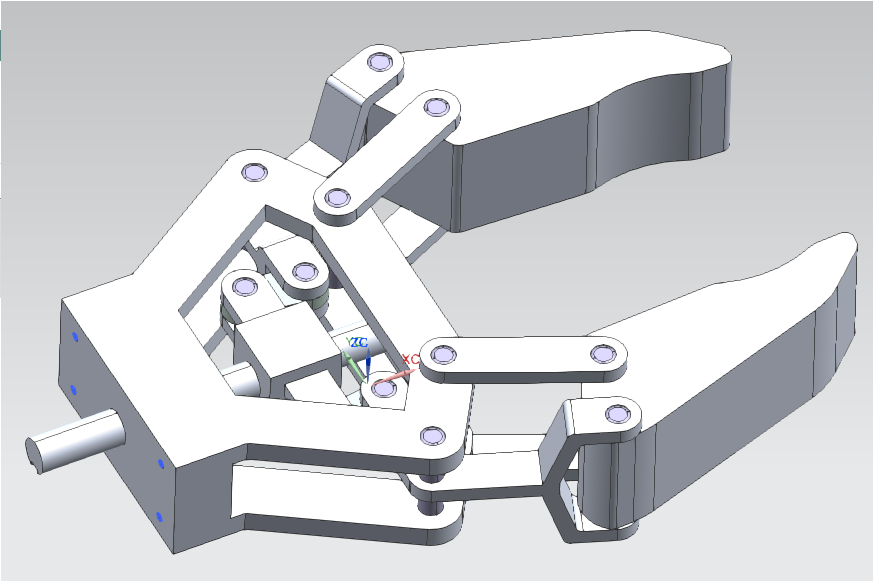
\includegraphics[scale=0.5]{Capitulo5/figs/Gripper.png}      %Ruta completa de la imagen, porque se compila desde el archivo tesis.tex
	\caption{Órgano Terminal}            %Pie de imagen
	\label{gripper01}                            %nombre de referencia
\end{figure}


\section{Ensamble de componentes}

\section{Sensores y actuadores}

\subsection{Motores}

\subsection{Decodificador óptico}

Para obtener datos que representen la posición y orientación de los eslabones se utiliza un deco

\section{Microcontrolador}